% (c) GreenSocs Ltd
% author: Christian Schroeder <schroeder@eis.cs.tu-bs.de>

%%%%%%%%%%%%%%%%%%%%%%%%%%%
%%%%%%%%%%%%%%%%%%%%%%%%%%%
%%%%%%%%%%%%%%%%%%%%%%%%%%%
\newpage
\section{Tutorial Full Example}

Figure \ref{fig:gavdemoplatform} shows an overview of the demonstration platform we use in this tutorial. A sample implementation is in the directory \Verzeichnis{greencontrol/examples/gav\_demonstration\_platform}. The modules are:
\begin{itemize}
	\item \textsl{Random traffic generators (TG1, TG2, TG3)}: Acts as bus
masters and create test traffic to the memory and the PCIe devices. Their
behavior can be set with configurable parameters (and can be changed even during runtime).
	\item \textsl{Caches (Cache1, Cache2, Cache3)}: This caches are write-back LRU caches whose size and line size is configurable during runtime. They also can be disabled during runtime.
	\item \textsl{Router\_SimpleBus}: The router is modeled by the SimpleBus router and needs not be developed as user module.
	\item \textsl{Memory (Mem)}: This memory module is a simple double data rate random access memory (DDR RAM). It is a bus slave. Its size and base address should be configured.
	\item  \textsl{PCIe router (PCIeBridge\_SimpleBus)}: This is another SimpleBus router connected to the {\sffamily Router\_SimpleBus}.
	\item \textsl{PCIe devices (PCIeDevice1, PCIeDevice2)}: The functionality of these bus slaves is just a stub with registers which can be written and read. The base address should be configured.
\end{itemize}

\begin{figure}[H]
	\centerline{
		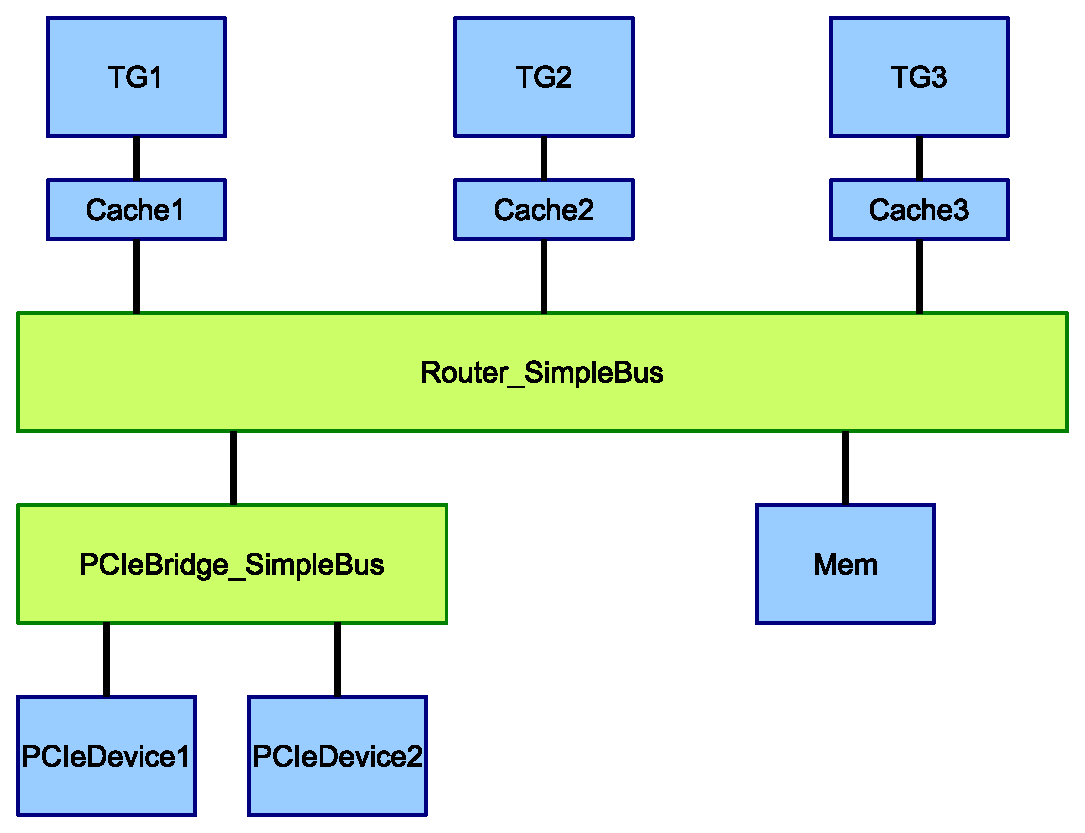
\includegraphics[width=15cm]{GAVDemoPlatform.eps}} 
	\caption{Analysis Demonstration Platform. }
	\label{fig:gavdemoplatform}
\end{figure}


%%%%%%%%%%%%%%%%%%%%%%%%%%%
\subsection{Analysis features}

This is a list of the analysis features this demo platform provides:

\begin{itemize}

% TODO: list parameter names where to access the analysis results!

   \item  {\em Cache hit rates:} \newline
  	\Datei{greencontrol/examples/analysis\_demonstration\_platform/lru\_cache.*} \newline
	Each cache provides two hit rate analysis parameters:
	\begin{itemize}
	  \item  Overall hit rate 
	  \item  Hit rate of a specific address range.
	  	The address range can be specified using configurable parameters of this module:
		{\sffamily hitrate\_upper\_addr} and {\sffamily hitrate\_lower\_addr}. 
	\end{itemize}

   \item   {\em Transaction rates}: \newline
    \Datei{greenbus/protocol/SimpleBus/simpleBusProtocol.h} \newline
   	The SimpleBus protocol implementation provides several kinds of transaction rates:
		\begin{itemize}
		   \item Transactions per second over all ports, {\em extrapolated} to one second using
		the time between the first and the last transactions that were ever 
		recorded in this simulation. Updated on each transaction. Does not show the utilization 
		over time but the overall utilization of the ports.
	   \item  Transactions per second for each in and out port ({\em extrapolated} version). Same 
	   	as transactions per second over all ports but separately for each port.
	   \item  {\em Dynamic} transactions per second over all ports, counting the actual
			transactions that were transmitted in the last second. Updated at the 
			end of each second. Can be outputted to show the utilization over time
			(with a granularity of one second).
	%\item \TODO:  {\em Dynamic} transactions per second for each in and out port.
	%	 \textcolor{red}{(may be left out for demo, TODO for later)} % TODO
		\end{itemize}
		
   \item   {\em Transaction latency}: \newline
		\Datei{greenbus/api/simplebusApi.h}  \newline
		The SimpleBus master port (API) provides two kinds of transaction latencies. The resulting value
		is the double representation of sc\_time.
      \begin{itemize}
          \item  {\em Transaction overall latency} (in the master port):    
          		Time a transaction needs between sending (in the master) 
			and completion (in the master).
	   \item  {\em Transaction transport latency}:
			Time the request needs to be sent by the master and acknowledged by the slave
		(phases {\sffamily Request} and {\sffamily RequestAccepted}), measured in the SimpleBus master port.
       \end{itemize}
       
   \item  {\em Transaction recording}: \newline
	\Datei{greenbus/api/simplebusApi.h} (in the slave port) \newline
	Transaction recording can be switched on / off with a configurable parameter.
	Filtering to record transactions of only one master can be enabled by setting a configurable 
	parameter to a master ID. \newline
	{\em Note} that this transaction recording is an example and insists not on well performing 
	and beautiful implementation.
   	
%   \item \TODO {\em Visible registers and memory}: \newline
%      \begin{itemize}
%        \item  \TODO {\em Visible PCIe registers}: The memory of the PCIe devices is visible because it is
%	      	made of \lstinline|gs_param|s. 
%		\textcolor{red}{(maybe leave this out because visible memory will be added later with drf?)}
%        \item  \TODO {\em Visible memory content}: The memory of the {\sffamily Mem} device is visible because it is
%       	 	made of \lstinline|gs_param|s.
%			\textcolor{red}{(maybe leave this out because visible memory will be added later with drf?)}
%      \end{itemize}
   	
\end{itemize}

To not influence the GreenBus as it is without GreenControl, all changes for analysis are surrounded by \lstinline[language=TeX]|#ifdefs GAV_ENABLED| and \lstinline[language=TeX]|#endif|. {\sffamily GAV\_ENABLED} is defined in the demo platform's global include file (\Datei{demo\_globals.h}) which is included in each file before including anything else. 


%%%%%%%%%%%%%%%%%%%%%%%%%%%
%%%%%%%%%%%%%%%%%%%%%%%%%%%
\section{Analysis Examples}

This section picks up the most important parts of the analysis features and describes them in more detail. These examples show how analysis framework can be used, but they demand not to be complete. The later examples only handle new elements and do not repeat issues discussed in previous analysis examples.


%%%%%%%%%%%%%%%%%%%%%%%%%%%
\subsection{Overall Hit Rate Statistics Calculator}

See file \Datei{greencontrol/examples/analysis\_demonstration\_platform/lru\_cache.*}

The overall hit rate Statistics Calculator calculates the hit rate within a cache.

Since the cache class registers callbacks it calls the macros \lstinline|GC_HAS_CALLBACKS();| (in the body) and \lstinline|GC_UNREGISTER_CALLBACKS();| (in the destructor).

Two configurable parameters (\lstinline|gs_param|s) are used to count the overall hits and misses. They are incremented each time a cache hit or miss occurs. The incrementation is independent on the calculation done within the StatCalc and is done even if it is disabled.
\begin{lstlisting}
  gs::gs_param<unsigned int> overall_hits;
  gs::gs_param<unsigned int> overall_misses;
\end{lstlisting}

The class member pointer to the StatCalc \newline
\lstinline|gs::av::StatCalc<double> *overall_hit_rate;| \newline
allows to delete the StatCalc and its Calculator in the destructor:

\begin{lstlisting}
delete overall_hit_rate->get_calculator();
delete overall_hit_rate;
\end{lstlisting}

\begin{itemize}
	\item  The calculator can be deleted before the StatCalc object. In this case the (default) trigger will be delete automatically by the StatCalc destructor. When instantiating a separate trigger, it must not be deleted before the StatCalc!
\end{itemize}

In the constructor the following Statistics Calculator (StatCalc) is created:
\begin{lstlisting}
  // Overall hit rate Statistics Calculator
  gs::av::Calculator<double> *hr_calc // Create Calculator
    = new gs::av::Calculator<double>("overall_hit_rate");
  hr_calc->enable_sloppy(); // allow division by zero
  // prepare parameters for convenience operators
  gs::gs_param_base& hits   = overall_hits;
  gs::gs_param_base& misses = overall_misses;
  // set formula: 100*(hits / (hits+misses))
  hr_calc->calc("*", 100, (*hr_calc)(hits / (*hr_calc)(hits + misses))); 
  // create Statistics Calculator
  overall_hit_rate = 
    new gs::av::StatCalc<double>("overall_hit_rate", hr_calc); 
  cout << "overall_hit_rate parameter name: " 
    << overall_hit_rate->get_result_param()->getName() << endl;
\end{lstlisting}

\begin{itemize}

	\item  Both, the Calculator (lines 2-3) and the StatCalc (lines 11-12), are {\em templated} to double. This means all results and intermediate results and calculations will be done using and returning the data type double. Never use two different templated classes here!

	\item  The Calculator is made {\em sloppy} (line 4) to ignore divisions by zero.
	
	\item  The Calculator's {\em formula} is set in line 9 with a mix of {\em convenience syntax} and {\em standard syntax}. For the convenience syntax the input parameters are casted to \lstinline|gs_param_base|s (lines 6-7). The standard syntax is used for the multiplication because the convenience syntax does not support constants (\lstinline|100|).
	
	 \item The StatCalc is created in lines 11-12. There a {\em default trigger} will be created implicitly which triggers on each change of the formula input parameters (hits, misses).
	 
	 \item The {\em result parameter} can be accessed by calling \lstinline|get_result_param()|.
	
\end{itemize}

Needed includes are:
\begin{lstlisting}
// GreenControl and GreenConfig
#include "greencontrol/gcnf/apis/gs_param/gs_param.h"
// GreenAV
#include "greencontrol/gav/apis/gav_api/GAV_Api.h"
#include "greencontrol/gav/plugin/StatCalc.h"
\end{lstlisting}


%%%%%%%%%%%%%%%%%%%%%%%%%%%
\subsection{Extrapolated Transactions per Second}

See file \Datei{greenbus/protocol/SimpleBus/simpleBusProtocol.h}

The GreenBus SimpleBus protocol has been extended to provide transactions per second statistics.

The needed analysis include is:
\begin{lstlisting}
#include "greencontrol/gav/plugin/StatCalc.h"
\end{lstlisting}

A global static function is added for {\em special calculation needs} to be added to the double Calculator class:
\begin{lstlisting}
/// Average calculator function to be added to the Calculator<double>
static double per_second(double transaction_count, 
                         double start_time_in_seconds, bool sloppy) {
  return (transaction_count / 
                (sc_time_stamp().to_seconds() - start_time_in_seconds));
}
\end{lstlisting}

A class member parameter is used to count all transactions:
\begin{lstlisting}
gs::gs_param<unsigned int> tr_cnt;
\end{lstlisting}

The class member pointer to the StatCalc (\lstinline|*overall_tr_per_sec|) allows to delete the StatCalc and its Calculator in the destructor.

Within the protocol's constructor this code creates the StatCalc:
\begin{lstlisting}
// Add user defined calculation function to Calculator class
gs::av::Calculator<double>::addFunc(&per_second,"per_second"); 
    
gs::av::Calculator<double> *trpsec_calc
  = new gs::av::Calculator<double>("tr_p_sec_overall");
trpsec_calc->enable_sloppy(); // allow division by zero
// set formula: (tr_cnt 'per seconds')
trpsec_calc->calc("per_second", tr_cnt, sc_time_stamp().to_seconds()); 
// create Statistics Calculator
overall_tr_per_sec = new gs::av::StatCalc<double>("overall_trans_per_sec_StC", trpsec_calc); 
cout << "transactions per second parameter name: " << overall_tr_per_sec->get_result_param()->getName() << endl;
\end{lstlisting}

\begin{itemize}

	\item  All analysis related code in the SimpleBus protocol is {\em guarded} by a \lstinline[language=TeX]|#ifdef GAV_ENABLED| which has to be enabled by the simulation including the GreenBus.

	\item  The {\em new calculation function} \lstinline|per_second| is added to the Calculator$<$double$>$ class (line 2) with the access string ``per\_second''.
	
	\item  The current sc\_time\_stamp is used as a constant (using the to\_seconds() function) (line 8).

\end{itemize}


Extrapolated transactions per second for each in and out port work the same. For each port one counter parameter and one StatCalc is created.

%%%%%%%%%%%%%%%%%%%%%%%%%%%
\subsection{Dynamic Transactions per Second}

See file \Datei{greenbus/protocol/SimpleBus/simpleBusProtocol.h}

A class member static function is added with special functionality: A function-internal static vector stores old values for each protocol instance. The second function parameter is used to identify the protocol instance because the calculation itself only needs one input parameter -- the transaction counter. The function calculates the transaction count between the current call and the last call to this function. This function should be called once per simulated second to deliver a transactions per second value that is {\em dynamically updated}.
\begin{lstlisting}
  static unsigned int transaction_count_diff(unsigned int transaction_count, unsigned int protocol_inst_no, bool sloppy) {
    static vector<unsigned int> old_values;
    if (old_values.size() < protocol_inst_no+1) old_values.resize(protocol_inst_no+1);
    unsigned int diff = (transaction_count - old_values[protocol_inst_no]);
    old_values[protocol_inst_no] = transaction_count;
    return diff;
  }
\end{lstlisting}

The protocol instance number is incremented with a static member function.

\begin{lstlisting}
    // Add user defined calculation function to Calculator class
    gs::av::Calculator<unsigned int>::addFunc        (&SimpleBusProtocol::transaction_count_diff, "private_transaction_count_diff"); 

    // Formula Calculator
    gs::av::Calculator<unsigned int> *dy_trpsec_calc
      = new gs::av::Calculator<unsigned int> ("dynamic_tr_p_sec_overall");
    dy_trpsec_calc->
      calc("private_transaction_count_diff", tr_cnt, getInstNumber());
    // Trigger
    gs::av::Trigger *dy_tr = new gs::av::Trigger(1, SC_SEC);
    // StatCalc
    dy_overall_tr_per_sec = new gs::av::StatCalc<unsigned int> ("dynamic_overall_trans_per_sec_StC", dy_tr, dy_trpsec_calc);
\end{lstlisting}

\begin{itemize}
	\item  The {\em trigger} (line 10) triggers the calculation each 1 SEC.
	\item  The StatCalc gets the Calculator and the Trigger as a parameter (line 12).
\end{itemize}

The trigger has to be deleted in the destructor (together with the Calculator and StatCalc). The trigger must be deleted {\em after} the StatCalc object:
\begin{lstlisting}
// do not delete the trigger before deleting the StatCalc!!
delete dy_overall_tr_per_sec->get_calculator();
gs::av::trigger_if* t = dy_overall_tr_per_sec->get_trigger();
delete dy_overall_tr_per_sec;
delete t;
\end{lstlisting}


%%%%%%%%%%%%%%%%%%%%%%%%%%%
\subsection{Transaction Latency}

See file \Datei{greenbus/api/simplebusApi.h} (master port).

The SimpleBus master port provides a time measurement for the overall (and transport) transaction latency. This example shows the overall latency.

All analysis features are guarded with a \lstinline[language=TeX]|#ifdef GAV_ENABLED|.

The needed includes are:
\begin{lstlisting}
#include "greencontrol/gcnf/apis/gs_param/gs_param.h"
#include "greencontrol/gav/plugin/StatCalc.h"
\end{lstlisting}

Class member parameters are used to store the transaction start and end time points, which are used as input parameters to a StatCalc.

\begin{lstlisting}
// Formula Calculator
gs::av::Calculator<double> *tr_overall_latency_calc
  = new gs::av::Calculator<double>("transaction_overall_latency");
tr_overall_latency_calc->calc("-", transaction_overall_latency_end_timepoint, transaction_latency_start_timepoint);
// Trigger
std::vector<gs::gs_param_base*> 
  sensitive_params(1, &transaction_overall_latency_end_timepoint);
gs::av::Trigger *tr = new gs::av::Trigger(sensitive_params);
// StatCalc
tr_overall_latency = new gs::av::StatCalc<double>
  ("transaction_overall_latency_StatCalc", tr, tr_overall_latency_calc);
\end{lstlisting}

\begin{itemize}
	\item  The trigger takes changes of only one of the formula input parameters as a trigger event (``{\em manually chosen parameters}'') (line 8). The trigger parameters have to be given as a vector of parameter bases (lines 6-7).
	
	\item On each start point of a transaction \newline 
	\lstinline|transaction_latency_start_timepoint = sc_time_stamp();|\newline
	is changed to the current time stamp. At this point {\em no} calculation is done because the trigger only triggers on changes of the end point parameter!
	
	\item  On each end point of a transaction \newline
	\lstinline|transaction_overall_latency_end_timepoint = sc_time_stamp();| \newline
	is changed to the current time stamp. On this change the trigger triggers the calculation and the difference between the end and the start point is outputted as the result.

\end{itemize}

The destructor deletes the Calculator, the StatCalc and the Trigger: \newline
\noindent
\begin{minipage}{\textwidth}
\begin{lstlisting}
delete tr_overall_latency->get_calculator();
gs::av::trigger_if* tr = tr_overall_latency->get_trigger();
delete tr_overall_latency;
delete tr;
\end{lstlisting}
\end{minipage}

The {\em transaction transport latency} works exactly the same with the difference that another end point parameter is used which is changed when the request of the transaction has finished. The same start point parameter is used!


%%%%%%%%%%%%%%%%%%%%%%%%%%%
\subsection{Transaction Recording}

See file \Datei{greenbus/api/simplebusApi.h} (slave port).

The GreenBus Generic transactions can be recorded at the SimpleBus slave port.
{\em Note} that this transaction recording is an example and insists not on well performing 
	and beautiful implementation.
	
This include is needed. This is a specialization for the gs\_param class which is specialized to the class GenericTransactionCopy. This copy class allows a transactions to be assigned to the copy class. The most important attributes will then be copied to this copy object. This is much overhead, not suitable for productive systems!
\begin{lstlisting}
#include "greencontrol/gcnf/apis/gs_param/gs_param_GenericTransactionCopy.h"
\end{lstlisting}

A class member parameter allows to enable or disable the recording:
\begin{lstlisting}
gs::gs_param<bool> record_transactions_enabled;
\end{lstlisting}
This parameter may be set during construction to enable the recording for that port. (The default is disabled.)

A class member parameter
\begin{lstlisting}
gs::gs_param<gs::cnf::GenericTransactionCopy> recorded_transaction;
\end{lstlisting}
is used as the parameter that can be outputted by the user to an {\em output plugin} like this (part of user code, e.g. testbench):
\begin{lstlisting}
#include "greencontrol/gav/plugin/File_OutputPlugin.h"
// ** Analysis file-output for recorded transactions at Mem slave port
gs::av::OutputPlugin_if* record_opp 
  = mainGAVApi->create_OutputPlugin(gs::av::FILE_OUTPUT_PLUGIN, "recorded_transactions.log.txt");
// add recorded transaction to file output
gs::gs_param_base *recorded_mem_transaction = mainApi->getPar("Mem.simplebus_slaveport.recorded_transaction");
mainGAVApi->add_to_output(record_opp, recorded_mem_transaction);
\end{lstlisting}

\begin{itemize}
	\item  The needed output plugin file has to be included.
	\item  An {\em output plugin} is created (lines 1-2) using the specified file name to output a human-readable file.
	\item  The output parameter of the slave port is added to this output plugin (line 6).
\end{itemize}

Additionally the slave port allows to record transactions only from a specific master. For this the class member parameter
\begin{lstlisting}
gs::gs_param<long> record_transaction_master_id_filter;
\end{lstlisting}
can be set by the user, e.g. (part of user code, e.g. testbench):
\begin{lstlisting}
  // only record transactions from the master Cache1
  gs::gs_param<long> *record_transaction_master_id_filter 
    = dynamic_cast<gs::gs_param<long>*>(
      mainApi->getPar
        ("Mem.simplebus_slaveport.record_transaction_master_id_filter"));
  *record_transaction_master_id_filter = cache1.master_port.get_master_port_number();
\end{lstlisting}
The default is ``0''. Then all transactions are recorded.

A transaction is recorded using this code within the slave port:
\begin{lstlisting}
// Analysis: record write transaction
if (record_transactions_enabled) {
  if (record_transaction_master_id_filter == 0
      || record_transaction_master_id_filter == ah->getMID())
    recorded_transaction = *(ah.get());
}                  
\end{lstlisting}
